\documentclass[a4paper,11pt,onecolumn,twoside]{article}
% 编译方式:xelatex三次编译
\usepackage{ctex}
\usepackage{fancyhdr}
\usepackage{amsmath,amsfonts,amssymb,graphicx}
\usepackage{subfigure}
\usepackage{indentfirst}
\usepackage{bm}
\usepackage{multicol}
\usepackage{indentfirst}
% \usepackage{picins}
\usepackage{abstract}
\usepackage[T1]{fontenc}
\usepackage{mathptmx}
\usepackage{float}
\usepackage{graphicx}
\usepackage{stfloats}
\usepackage{mdframed}
\usepackage{amsmath}
\usepackage{authblk}
\usepackage{epstopdf}
\usepackage{caption2}
\usepackage{subfigure}
\usepackage{hyperref}
\usepackage{paralist}
\usepackage{wallpaper}
\usepackage[algo2e,ruled,vlined]{algorithm2e}
\hypersetup{
    colorlinks=true,
    linkcolor=blue,
    filecolor=blue,
    urlcolor=blue,
    citecolor=black,
}

\addtolength{\topmargin}{-54pt}
\setlength{\oddsidemargin}{-0.9cm}
\setlength{\evensidemargin}{\oddsidemargin}
\setlength{\textwidth}{17.00cm}
\setlength{\textheight}{24.00cm}

\newcounter{TempEqCnt}
\renewcommand{\baselinestretch}{1.1}
\parindent 22pt

\begin{document}
\title{\huge{直肠全系膜切除非传统术式综述}}

\author[]{曾树新}{}
\author[]{赵子毅}{}
\author[]{王美璇}{}
\author[]{陈春霖}{}
\author[]{李易霖}{}
\author[]{季树宇}{}

\affil[]{深圳大学医学部临床医学专业}
\affil[]{\textit {\{2018221146, 2018221138, 2018221088, 2018221020, 2018221091, 2018221092\}@email.szu.edu.cn}}


\renewcommand\Authands{ 和~ }


\date{}

\CenterWallPaper{1}{img/logo.png}

\fancypagestyle{plain}{
    \fancyhf{}
    \rhead{\thepage}
    \chead{\centering{局部解剖学期末论文\\
            \scriptsize{\textbf{Local anatomy}}}}
    \lhead{Jan, 2021}
    \lfoot{}
    \cfoot{}
    \rfoot{}
}

\pagestyle{fancy}
\fancyhf{}
\headheight 26.70523pt
\fancyhead[LE,LO]{Jan, 2021}
\fancyhead[CE,CO]{局部解剖学期末论文}
\fancyhead[RE,RO]{\thepage}
\lfoot{}
\cfoot{}
\rfoot{}

\newenvironment{figurehere}
{\def\@captype{figure}}
{}
\makeatother

\maketitle

\newcommand{\supercite}[1]{\textsuperscript{\cite{#1}}}


\setlength{\oddsidemargin}{1cm}  % 3.17cm - 1 inch
\setlength{\evensidemargin}{\oddsidemargin}
\setlength{\textwidth}{13.50cm}
\vspace{-.8cm}
\begin{center}
    \parbox{\textwidth}{
        \textbf{摘~~~要} \quad  直肠癌是常见的消化道恶性肿瘤之一,近年来在全球范围内,直肠癌的发病和死亡呈明显上升趋势,发病年龄有所提前。由于我国居民生活饮食结构的改变及人口老龄化进程加快,近年来我国结直肠癌的发病和死亡均呈上升趋势。在我国,直肠癌的特点之一是低位直肠癌为主,对直肠癌的外科治疗提出了新的挑战。随着人们对生活质量的要求提高及外科微创化概念的深入推广,新的直肠癌切除术——直肠系膜经肛内镜全切除术(TaTME)以更清晰的腔镜视野、更精确的控制、更大的操作空间、更好的保护健康组织、更少的并发症获得越来越多的青睐。本文通过对直肠解剖结构、直肠癌、传统术式——开腹、经腹壁腔镜的介绍及新旧术式的比较对经肛内镜全切除术进行综述。
        \\
        \textbf{关键词} \quad 直肠癌,TaTME,外科治疗,医学}
\end{center}

\vspace{.1cm}
\begin{center}
    \parbox{\textwidth}{
    \begin{center}
        {\large{\textbf{Total mesorectum resection is not a traditional surgical review}}}\\[4pt]
        \vspace{-0.5cm}\end{center}
    \begin{center}
        \textbf{Zhao Ziyi, Zeng Shuxin, Wang Meixun, Chen Chunlin, Li Yilin, Ji Shuyu}\\[2pt]
        \small{\textit{(Health Science Center of Shenzhen University)}}\\[2pt]
    \end{center}
    {\small{\textbf{Abstract}\quad Rectal cancer is one of the common malignant tumors of the digestive tract. In recent years, the incidence and death of rectal cancer have been on the rise globally, and the age of onset has advanced. Due to the changes in the dietary structure of Chinese residents and the accelerated process of population aging, the incidence and death of colorectal cancer in my country have also been on the rise in recent years. In my country, one of the characteristics of rectal cancer is low rectal cancer, which poses new challenges to the surgical treatment of rectal cancer. With the improvement of people’s requirements for the quality of life and the in-depth promotion of the concept of minimally invasive surgery, the new rectal cancer resection-mesorectal transanal endoscopic resection (TaTME) has a clearer endoscopic vision and more precise Control, larger operating space, better protection of healthy tissue, and fewer complications are gaining more and more favor. This article reviews the anatomical structure of the rectum, rectal cancer, traditional surgical methods-laparotomy, transabdominal endoscopy, and comparison of the new and old surgical methods.
        \\
        \textbf{Key Words}\quad Rectal cancer, TaTME, Surgical treatment, Medicine}}
    }
\end{center}

\setlength{\oddsidemargin}{-.5cm}
\setlength{\evensidemargin}{\oddsidemargin}
\setlength{\textwidth}{17.00cm}

\vspace{0.2cm}
\begin{multicols}{2}

    \section{前言与介绍}
    盆腔脏器主要包括泌尿器、生殖器及消化管的盆腔部分。直肠位于真性骨盆内,由平第三骶椎,即乙状结肠系膜终止处由乙状结肠移行为直肠,随后向下穿过盆膈下接肛管,形成下消化道的一部分。

    \subsection{直肠}

    \noindent\textbf{位置}~~直肠上份平第三骶椎,与骶骨、尾骨、梨状肌相靠近,两者之间存在疏松的结缔组织,内有骶丛、盆内脏神经、直肠上动静脉等结构。直肠两侧有直肠侧韧连接至盆腔侧壁,其中有直肠下血管、盆内脏神经走行,韧带后方有盆丛、髂内动静脉经过。直肠前隔着直肠膀胱隔与膀胱、女性子宫等器官相毗邻,并形成直肠膀胱陷凹、直肠子宫陷凹等腹腔直立体位最低点,具有重要的临床意义。

    \noindent\textbf{结构}~~直肠由乙状结肠移行而来,形成直肠壶腹,直肠壶腹向下延续为3个直肠弯曲,有直肠内的3条横襞所形成,再向下便通过肛直肠线与肛管相分隔。

    \noindent\textbf{血管}~~直肠可由三条动脉分别供应直肠的不同区域:1)来自肠系膜上动脉延续——直肠上动脉,分布血流到直肠的左右;2)来自髂内动脉前干脏支的直肠下动脉,分布血流到直肠下部;3)来自骶外侧动脉与骶正中动脉形成的梯形血管网发出的终末0至3条直肠分支供血,分布血流到直肠后壁。直肠的静脉多与动脉同名且伴行,且多汇合成网,如浆膜下层有直肠肛管外丛、粘膜下有直肠肛管内丛。前者回流入髂内静脉,后者通过肠系膜上静脉回流入门静脉,形成门腔静脉的交通血管。

    \noindent\textbf{淋巴结}~~直肠上下部分分别可通过直肠上淋巴结及直肠旁淋巴结、髂内淋巴结与机体淋巴结相沟通,当发生癌症时,可分别引起上行性转移和下行性转移,直肠上部分的癌细胞可以由于淋巴液的流动方向的改变而发生逆行性向下转移。侧方淋巴结属第三站淋巴结,如果受侵表示已属晚期,即使清扫了预后亦仍不佳。而无受侵者,预防性扩大清扫更无必要\supercite{DIWEI}。

    \noindent\textbf{神经}~~特别的是,左半结肠以下副交感神经来自盆内脏神经,在直肠处可支配排便。同时直肠癌时,癌组织若是浸润至骶丛,可引起剧烈疼痛。

    \subsection{直肠癌}
    直肠癌可通过腹膜折返的位置分为上段直肠癌和下段直肠癌,中国人的直肠癌的发病率要比结肠癌高,且下段直肠癌发病率更高,这也为直肠系膜经肛内镜全切除术(TaTME)的国内应用赋予了合理性。直肠癌主要分为腺癌、腺鳞癌、未分化癌,可通过TNM,也就是肿瘤侵犯严重程度、淋巴结转移、远处转移进行分期。直肠癌的转移方式主要是通过淋巴结转移,同时亦可通过血行转移达肝脏、肺部、脑部。目前临床上常见的直肠癌征象是指诊肿块、腹股沟淋巴结肿大、肠梗阻相关症状,大便隐血、癌胚抗原、内镜检查、影像学检查等辅助方式进行确诊,多数使用手术、放射性治疗、化疗的方式治疗,也可以通过烧灼、激光、冷冻治疗的方式进行治疗。

    \subsection{外科治疗}
    传统外科方法有——开腹TME,全称:直肠癌与开腹直肠全系膜切除,采用下腹部正中绕脐切口。分离乙状结肠左侧及右侧系膜,两边在腹膜返折处会师,而后在直视下结扎肠系膜下血管并清扫相应部位淋巴结。然后,在行盆腔内直肠的游离后,采用闭合器或荷包钳切断直肠。最后用管状吻合器进行肠管吻合\supercite{1}。

    \begin{figure}[H]
        \centering
        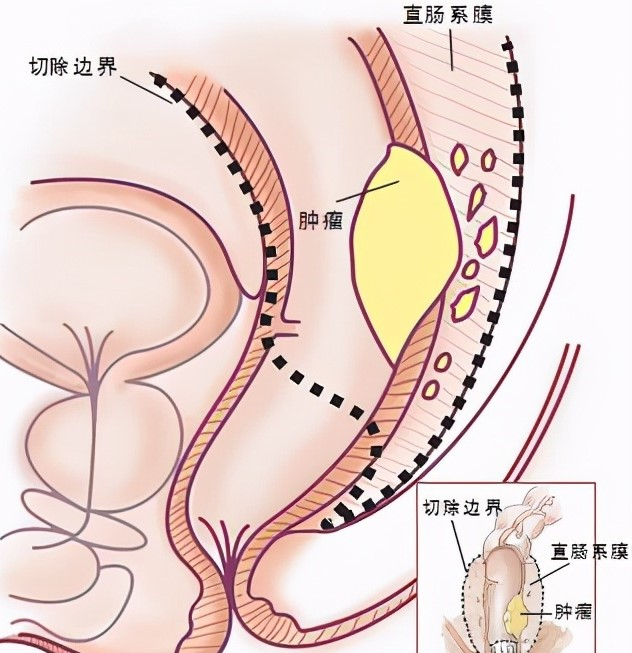
\includegraphics[width=\linewidth]{img/r.jpg}
        % \begin{algorithm2e}
        \caption{直肠全系膜切除范围示意图}
        % \end{algorithm2e}
        \label{DNN}
    \end{figure}

    \section{腹腔镜TME}
    腹腔镜TME,全称:腹腔镜直肠全系膜切除,主要是由腹腔镜直肠前切除术(LAR)、腹腔镜腹会阴联合切除术(APR)\supercite{2}两部分组成。如遇肿瘤过大或广泛浸润导致腹腔镜下不能切除,或肿瘤切缘不充分,抑或大量出血者等,应中转行开腹TME。
    \subsection{经腹直肠切除吻合术(LAR)}
    LAR不但保留了肛管和肛提肌,并且也保留了直肠下段的感觉及其排便反射(保留下段长度在4~5cm以上时),故为直肠切除术中保留排便控制功能效果最好的手术,术后病人逐渐多能恢复控制和排气的能力。适用于直肠中、上段癌。

    病人取头低足高30°的膀胱截石位,分离乙状结肠系膜的右侧,,切断肠系膜下动脉或直肠上动脉及其伴行静脉。沿着直肠固有筋膜与盆壁筋膜的间隙行锐性分离,低位直肠肿瘤的骶前分离应至尾骨尖部。切开直肠前腹膜返折,于Denonvillier筋膜之间的间隙将直肠前壁与精囊分离(女性在直肠生殖膈平面与子宫及其附件进行分离)。切断两侧的侧韧带并注意保护盆腔的自主神经。在肿瘤下方3cm处用腹腔镜切割缝合器切断直肠。在下腹作相应大小的小切口,将带肿瘤的近端直肠乙状结肠拉出腹腔外,切除肠段。将圆形吻合器抵钉座放入近端结肠,重新建立气腹,使用吻合器在腹腔镜直视下作乙状结肠-直肠端端吻合。

    \subsection{腹腔镜腹会阴联合切除术(APR)}
    APR是根治性手术,患者需在腹部行人工肛门造口排便。适用于直肠下段及肛管癌和某些无条件作保留肛门的直肠中段癌病人\supercite{3}。

    在腹主动脉前开腹,游离、切断肠系膜下动脉或乙状结肠动脉及其伴行静脉。分离结肠系膜,将乙状结肠系膜从后腹膜壁游离。游离直肠,切除两侧韧带,在腹腔内用线形切割器或体外直接切断乙状结肠,在左下腹适当位置作腹壁造口。肛门需作双重荷包缝合。环绕肛门作皮肤梭形切口,切断肛尾韧带,在两侧靠近盆壁处分离并切断肛提肌。剪断直肠前的附着肌肉,将直肠切除。

    柱状经腹会阴切除术(肛提肌外腹会阴切除术)是一种新出现的新术式\supercite{4},较常规经腹会阴切除术可以切除更多的癌周组织,减少术中穿孔,降低环周切缘阳性率,从而达到改善预后的目的。

    \section{TaTME}
    TaTME,全称:直肠系膜经肛内镜全切除,是近年来出现的一种自然腔道内镜手术,较传统的开放及腹腔镜手术微创美观。国际上首例临床应用由美国学者Sylla\supercite{5}等于2009年底施行,亚洲首例临床应用则由陈光远于2010年5月施行,此后有多国专家在临床应用报道中较多论证了该术的可行性和安全性\supercite{6,7,8},但是在对肿瘤根治术来说最重要的根治性方面缺乏全面评价。

    \subsection{适应症}
    \begin{compactenum}
        \item 直肠腺瘤或复发性腺瘤,包括无蒂广基型和绒毛状腺瘤,一般瘤体最大占直肠周径的3/4以内\supercite{9,10}。
        \item T1期低复发危险直肠癌,指肿瘤高分化、中分化,瘤体小,活动度大的T1期直肠癌,其淋巴转移率为3\%-5\%,已普遍接受为TaTME的适应证。
        \item T1高危癌,即癌累及不超过粘膜下层但组织分化达II、III级者,因其淋巴结累及的可能性增大,术后复发率增高,如行必须加用局部放、化疗,T1期低复发危险直肠癌合并有严重心脏病、慢性阻塞性肺病等常规根治术风险较大或拒绝腹壁肠造口者,术后可辅助放、化疗\supercite{11}。
        \item 任何高复发危险的直肠癌和T1期及T1期以上的直肠癌仅作为姑息手术,术后须辅以放疗、化疗。
        \item 继发于吻合术或肛瘘的直肠良性狭窄。
        \item 直肠脱垂。
        \item 直肠类癌和直肠阴道瘘。
    \end{compactenum}

    由于TaTME是新推广的局部切除术式,其适应征有一定争论。

    \subsection{手术操作及术后处理}
    对经严格选择的病人,术前必须作肠道准备。手术在全麻或脊髓麻醉下进行。病人的体位应根据肿瘤生长的部位而定,因为直肠镜前端斜口必须向下。所以,病灶位于直肠前壁则病人取胸膝位;位于后壁则取截石位;位于侧壁者则取侧卧位。常规会阴部消毒、铺巾,经轻柔扩肛后,选择适当长度的直肠镜经肛门插入,直视下调节到所需部位后固定于手术台上,正确连接各种配套装置,保持CO2低压充气状态,在立体视镜和腔镜系统下根据需要插入各种专用器械进行手术操作。首先围绕病灶黏膜下层注入1:100000肾上腺素,以使黏膜隆起和减少出血。充分暴露肿瘤后,用电刀在肿瘤边缘标记切除线。腺瘤的切距为0.5cm,并作粘膜下切除。大腺瘤、腺瘤局部变硬、术前组织学发现有不典型增生或高度怀疑恶变者,则切距为1cm,且须作肠壁全层切除。术前证实为癌,如肿瘤位侵犯浆膜,则除作肠壁全层切除外,尚须切除周围脂肪组织及其中淋巴结,直至骶前筋膜暴露。但位于直肠前壁的肿瘤,因前方邻近前列腺、尿道或阴道,应注意避免损伤周围重要组织器官,可行部分肠壁切除。女性病人因直肠腹膜返折低且水平不恒定,易误入腹腔或阴道,应特别注意。切除以电切为主,以保持术野清洁。手术创口予以腔内缝合:先在体外将一根7-10cm长带缝针的可吸收缝线的尾端夹一银夹,经直肠镜送人肠腔内,从创口一端开始,用特制的镊子和持针钳进行单层连续缝合,直至创口闭合,缝线另一端再用一银夹固定,剪下缝针并退出。如创口较大或缝合困难,可用多根缝线分次缝合。手术标本钉在硬板纸上标明方向及侧切缘,以便病理医师作出更准确的病理分析,以确定肿瘤的性质、切缘和淋巴结情况\supercite{12}。

    TaTME后患者一般无须特殊止痛处理,术后麻醉消退后嘱病人可自由活动,24小时后流质饮食。如无并发症2-3天后出院。出院后应定期在专科门诊随访。

    \subsection{TaTME禁忌证}
    T1期高复发危险或者更后期(如T2期或以上)的直肠癌,不以姑息治疗为目的则不适宜直接行该术。多发结直肠肿瘤是其禁忌症,术前应行全结肠镜、钡灌肠造影或多排螺旋CT结直肠重建等检查予以排除。腹膜返折以上直肠前壁肿瘤如采用TaTME行全层切除,容易切穿进入腹腔。TaTME须经肛门插入外径4CM的特殊直肠镜直至手术结束,可能会对肛门括约肌造成一定程度的影响。因此,肛门括约肌功能不良的患者不宜行TaTME,以免术后发生肛门失禁\supercite{13}。

    \subsection{TaTME并发症}
    由于TaTME操作精确,创伤小,对患者的全身影响甚小,因此手术并发症的发生率较低。

    \begin{compactenum}
        \item 一般并发症:一过性发热、腹泻、尿潴留、短暂性肛门出血(包括直肠创口渗血或扩肛引起的内痔出血),常能自行恢复。
        \item 直肠创口裂开:与创口张力过大或缝合技术缺陷有关。表现为术后肛门排出脓血性液,常伴发热。指检或结肠镜检查可确诊,多数可保守治愈。因直肠周围脂肪结缔组织尚完整,后果常较直肠前切除术后吻合口裂开要轻。
        \item 肛门直肠功能损害:TEM直肠镜直径达4cm,可致肛门括约肌过度拉伸。术后部分患者有暂时性肛门排气或排液态大便失禁,常于数天至三个月内恢复。
        \item 术中切穿肠壁至腹腔:在腹膜返折以上的腹膜面或乙状结肠作全层切除时易发生。如术中及时发现可在内镜下缝合修补,亦可中转开腹修补或行乙状结肠造口;若术后因腹腔内感染发现,则肠造口不可避免\supercite{14}。
        \item 其他并发症:对于女性患者,中下段直肠前壁切除过深亦可造成直肠阴道瘘。TaTME直接导致患者死亡的案例极其罕见\supercite{15}。
    \end{compactenum}

    \section{评价}
    自1991年报道了第一例因结肠良性肿瘤施行的腹腔镜右半结肠手术以来,腹腔镜在结直肠外科领域的应用便不断被人们探索。相比于传统的开放式手术,腹腔镜手术创伤小,术后恢复快,与外科领域逐步深入的微创理念相符合,因此得以快速发展。\supercite{W1}无论是吻合口漏还是中转开腹,发生率均与肿瘤位置息息相关。对于低位直肠癌患者来说,术野较差且暴露难度大,导致了肿瘤切缘无法保证等众多问题。TaTME因此产生,它通过肛门途径处理癌变组织,既不需要腹部切口又利用了天然孔道,符合现代内镜手术的思想。

    \subsection{腹腔镜TME评价}
    腹腔镜手术的发展思路,是在保持美观微创的同时,做到与开放式手术相同甚至更佳的临床疗效。同开腹手术一样,腹腔镜TME也要求遵循直肠全系膜切除术(TME)的手术要点,如高位结扎肠系膜血管,清扫足够的淋巴结,足够的远切缘和整块切除,保证环周切缘的完整性。\supercite{W4}腹腔镜TME已经可以做到与开腹TME手术复发率、无瘤生存率、总生存率差异均无统计学意义\supercite{W5}。在可进行手术的肿瘤大小、手术部位、术前、术后及手术器械冲洗液脱落肿瘤细胞等方面的比较上也无差异\supercite{16}。

    然而,腹腔镜TME存在中转开腹率、吻合口漏发生率高等风险,其术后并发症发生率是否低于开腹TME,也存在争议。值得注意的是,根据一些研究的大数据统计,腹腔镜TME与开腹TME比较,在多个方面都略次于开腹TME\supercite{17}。研究者及临床患者需要仔细考量这一研究结果。腹腔镜虽开口微小,但镜头可调节,放大手术视野,使解剖结构更清晰,更好地辨认盆筋膜脏、壁两层之间的疏松结缔组织间隙,理应更能识别和保护盆腔自主神经丛,完整地切除含脏层盆筋膜的直肠系膜,手术时间更短,术中出血量更少,并达到更好的根治效果。而且考虑到医师掌握腹腔镜手术有一定的学习曲线,如今的大多数术者对腹腔镜TME的掌握尚不熟练,大数据并不能鉴别医师的个人能力及水平及处于学习曲线发展中的哪一个阶段。所以,待医师完全掌握后,腹腔镜TME自然更优于开腹TME。

    有研究表明,随着腹腔镜TME的逐步应用与操作者经验的丰富,腹腔镜TME肿瘤切除的完整性已与开腹TME相似,腹腔镜低位直肠癌的环周切缘阳性率为9\%,明显优于开腹的22\%;腹腔镜TME的手术时间、术中出血率优于开腹TME,且切口感染、肺部感染、肠梗阻发生率明显更低\supercite{2,18};腹腔镜TME患者D术中出血量、术后下床活动时间、术后住院时间、肠鸣音恢复时间、术后止痛药应用次数均优于开腹TME患者\supercite{19,20};其清扫淋巴结数目也达到了与开腹TME相当\supercite{W3}。因此我们可以大致得出结论,虽然由于术者的掌握程度等原因,在大数据上腹腔镜TME可出现略逊于开腹TME的现象,腹腔镜TME仍然具有如上所述视野清晰,创伤小,疗效佳,并发症少以及安全性高的特点。

    值得注意的是,吻合口漏是直肠癌根治术后的严重并发症之一,且目前尚无很好的预防方法。吻合位置低是发生吻合口漏的危险因素,但目前腹腔镜TME对于低位结直肠癌的治疗效果并无明显优势,且需操作者经验十分丰富\supercite{W6}。中转开腹也是并发症发生率上升的危险因素,肥胖、肿瘤过大、局部病情较晚和术中出血较多是导致中转开腹的常见原因\supercite{W4}。因此,行腹腔镜TME需进行完善准确的术前评估与围术期准备,以期将中转开腹率降至最低。
    \subsection{TaTME评价}
    在2013年首例临床手术成功后,这一手术方式很快受到了临床研究一线的关注。这种手术方式通过癌变病灶远端开始,从下向上的方式进行操作,操作的角度较为合理,能够确保远端直肠游离操作的容易程度,同时还能够确保恶性肿瘤灶能够有足够的远端切缘。其可视图像是通过体现光学双目镜捕获的,视野深度大大改善,图像更加清晰,且针状电刀可保证切缘和切除深度得到较好的控制,因此切除精确,能够获取高质量的肿瘤标本用于准确的病理分期,能够达到有理想切缘的根治性切除效果,减少术后复发。TaTME无皮肤切口,可以避免不必要的开腹和肠造口术,手术时间短,创伤小,术中出血少,避免了背侧路径一些严重并发症,术后一般无需止痛治疗、恢复快,住院时间短,显然优于开腹TME。切除精确而无局部肿瘤残留,可切除距肛缘20cm以内的肿瘤,切除肿瘤完整,有利于组织学评价。是内镜、腹腔镜、显微手术的结合。同时,相比腹腔镜TME,逆向操作的方式不仅能够解决常规腹腔镜手术术野相对较差、低位直肠系膜暴露不足的问题,还可以充分暴露终末神经,避免手术损伤到盆腔神经系统,且手术后性功能损伤、尿潴留等并发症发生率较低\supercite{W8}。其次,由于特殊器械的设计使能够切除距肛缘4-25cm以内任何距离的直肠甚至远端乙状结肠的肿瘤,这是传统的TAR术、TSR术、TSLR术无法达到的。由于操作精确,创伤小,对患者的全身情况影响也甚小,手术并发症的发生率较低\supercite{W2,W6}。

    如果做一个横向比较,TaTME避免了经肛局部切除术(TAR)的手术要求肿物靠近肛门,显露不良,难掌握手术范围、深度的准确,不能对周围淋巴结清扫,不能很好的切除广基腺瘤或位于中、上直肠肿瘤的弊端;经骶局部切除术(TSR)需切除尾骨及部分骶骨,术野显露较差,术后易并发直肠皮肤瘘和伤口感染的弊端;经肛门括约肌切除术(TSLR)需全部切断肛门内外括约肌,创伤仍较大的弊端;经阴道局部切除术(TVR)适应症狭窄,且易发生直肠阴道瘘的弊端;内镜下黏膜切除术(EMR)切除体积较小(直径0.5-1.0mm),且经常采用肿瘤分块切除,导致术后肿瘤病理分期的困难,切除不彻底的弊端。

    但总的来说该术式还处于临床研究的阶段,作为近年来的新兴技术,仍有需要不断改进之处。一项挪威的研究结果显示,TaTME的环周阳性率较高,局部复发率高达9.5\%,远高于腹腔镜TME,原因可能与操作者的解剖知识与临床能力相关,该术式目前仍对肠系膜与血管的游离要求很高\supercite{W7}。

    \section{总结}
    在术者经过腹腔镜TME手术规范培训、具有TME经验技术的前提下,腹腔镜TME是安全可靠的直肠癌根治术式。对于很多医院,腹腔镜TME已经可以常规施行,并且有良好的发展前景。

    而TaTME的治疗思维和术式都是几乎全新的。无论是否Pure-NOTES,都在尝试根治切除的同时现微创美观效果的统一。工具的改良和技术的总结将让此术式获得更好的治疗效果和应用范围。在技术成熟后,这种新术式对于大多数患者,特别是低位或超低位的直肠癌患者,可以起到提高生活质量,同时降低术者的手术难度的效果。其“自下而上”的理念,是克服低位直肠及系膜难以探及的关键。一定程度上这提示了直肠癌手术发展的方向。
    \small
    \begin{thebibliography}{14}
        \setlength{\parskip}{0pt}  %段落之间的竖直距离
        %%% BIBTEX
        \bibitem{1}腹腔镜直肠癌手术与传统开腹直肠癌手术的疗效比较[J].秦光远,左朝晖,姚敦武,等.临床和实验医学杂志,2012,10(6):421-423.
        \bibitem{2}腹腔镜结肠直肠癌根治手术操作指南(2006版)[J].外科理论与实践.2006(05)
        \bibitem{3}经腹会阴联合切除术的回顾与发展[J].姜涛,刘彤,王鹏志山东大学学报(医学版).2020年05期
        \bibitem{4}肠癌柱状经腹会阴切除术[J].王振军.中华结直肠疾病电子杂志.2012(02)
        \bibitem{5}Sylla P,Rattner DW,Delgado S,et al.NOTES transanal rectal cancer resection using transanal endoscopic microsurgery and laparoscopic assistance[J].Surg. Endosc,2010,24(5):1205-1210.
        \bibitem{6}Emhoff IA, Lee GC, Sylla P. Transanal colorectal resection using natural orifice translumenal endoscopic surgery (NOTES [J]. Dig Endose, 2014, 26 (Suppl 1) : 29-42.
        \bibitem{7}Sylla P, Lacy AM. NOTES transanal rectal cancer resection using transanal endoscopic microsurgery [J]. Eur Surg, 2011,43(5) : 146-152.
        \bibitem{8}张浩,金雄伟,李满志,等完全经肛单孔腹腔镜全直系膜切除术治疗直肠癌[J].中国内镜杂志,2012,18(4):379-383.
        \bibitem{9}Platell C, Denholm E, Makin G. Efficacy of transanal endoscopic microsurgery in the management of rectal polyps. Gastroenterol Hepatol [J], 2004, 19: 767-772.
        \bibitem{10}Demartines N, von Flue MO, Harder FH. Transanal endoscopic microsurgical excision of rectal tumors: indications and results [J]. World J Surg, 2001,25: 870-875
        \bibitem{11}蒙家兴,林国乐,刘应裕.经肛门内镜显微手术治疗直肠绒毛状腺瘤和早期直肠癌31例,[J] 中国微创外科杂志2006年1月第6卷第1期,15-18.
        \bibitem{12}李克军,赵作伟,董播,等.经肛门入路腔镜下高位直肠类癌局部切除术(附6例临床报告). [J] 中国微创外科杂志2005年7月第5卷第7期,525-526.
        \bibitem{13}蒙家兴,邵初晓,刘应裕,等.经肛门内镜显微手术切除直肠肿瘤. [J] 中华胃肠外科杂志,2003年3月第6卷第2期,96-97.
        \bibitem{14}毕建军,邵永孚,高纪东.早期直肠癌的外科治疗,[J] 中国医刊,2004年39卷5期,25--26.
        \bibitem{15}王辉,直肠癌局部切除适应症及注意事项. [J] 肿瘤学杂志,2006年12卷1期,20--22.
        \bibitem{16}腹腔镜手术治疗结直肠癌安全性的临床研究[J].郑民华蔡景理陆爱国李健文王明亮董峰胡艳艳郁宝铭外科理论与实践.2003年05期
        \bibitem{17}结直肠癌研究30年回顾和现状[J].郑树张苏展黄彦钦实用肿瘤杂志2016,31(01)
        \bibitem{18}腹腔镜与开腹手术治疗结直肠癌的临床疗效及术后并发症的比较[J].朱渝军陈刚胡佳杨日高实用癌症杂志.2016年01期
        \bibitem{19}直肠癌治疗时采用腹腔镜手术与开放手术的疗效比较[J].范昌政,修福鋆.中国医药指南.2017(29)
        \bibitem{20}腹腔镜手术与开腹手术治疗结直肠癌临床效果比较的Meta分析[J].姜涛刘彤王鹏志中国全科医学.2011年05期


        \bibitem{DIWEI}郁宝铭. 低位直肠癌的诊治进展[J]. 中国实用外科杂志, 2002, 22(1):34-37.

        \bibitem{W1}孙学军,郑见宝.腹腔镜结直肠癌手术治疗研究进展[J].西安交通大学学报(医学版),2016,37(05):613-621.
        \bibitem{W2}朱渝军,陈刚,胡佳,杨日高.腹腔镜与开腹手术治疗结直肠癌的临床疗效及术后并发症的比较[J].实用癌症杂志,2016,31(01):103-106.
        \bibitem{W3}曹广,梁杰雄,王晓东.腹腔镜与开腹直肠癌根治术的疗效比较[J].中国微创外科杂志,2016,16(07):581-585.
        \bibitem{W4}王永鹏,佟昕,张庆彤,马思平,闫晓菲,李楠,孟庆凯,宋纯.腹腔镜直肠癌前切除术472例临床经验总结[J].中国微创外科杂志,2015,15(03):215-219.
        \bibitem{W5}李想,傅仲学,贾诩.腹腔镜与开腹全直肠系膜切除保肛术治疗低位直肠癌的Meta分析[J].重庆医学,2015,44(12):1658-1661.
        \bibitem{W6}覃华波,谢明颢,练磊,何晓生,吴小剑,兰平,汪建平.直肠癌根治术:腹腔镜与开腹手术后并发症的比较[J].中国普外基础与临床杂志,2015,22(05):530-534.
        \bibitem{W7}杜晓辉.腹腔镜结直肠手术进展及展望(2000-2020)[J].中国实用外科杂志,2020,40(02):191-194.
        \bibitem{W8}聂恒博,张春霞,高宏建.经肛与腹腔镜全直肠系膜切除术治疗直肠癌的临床疗效比较[J].临床和实验医学杂志,2020,19(05):534-537.

    \end{thebibliography}
    \normalsize

\end{multicols}


\clearpage

\end{document}
